\hypertarget{ForecastFile}{}
\section[Forecast File]{\protect\hyperlink{ForecastFile}{Forecast File}}
The specification of options for forecasts is contained in the mandatory input file named \texttt{forecast.ss}. See \hyperref[sec:forecast]{Forecast Module: Benchmark and Forecasting Calculations} for additional details. 

The term COND appears in the ``Typical Value'' column of this documentation (it does not actually appear in the model files) and indicates that the following section is omitted except under certain conditions, or that the factors included in the following section depend upon certain conditions. In most cases, the description in the definition column is the same as the label output to the ss\_new files.


\begin{landscape}
	
\hypertarget{fore-specify}{}
\subsection[Forecast File Options (\texttt{forecast.ss})]{\protect\hyperlink{fore-specify}{Forecast File Options (\texttt{forecast.ss})}}
  {
  \setlength\extrarowheight{4pt}	
  \begin{longtable}{p{2cm} p{7cm} p{12cm}} 
		
	\hline
	\textbf{Value} & \textbf{Options} & \textbf{Description} \Tstrut\Bstrut\\ 
	\hline
	\endfirsthead
		
  \hline
	\textbf{Value} & \textbf{Options} & \textbf{Description} \Tstrut\Bstrut\\ 
	\hline
	\endhead
		
	\hline
	\endfoot
		
	\hline
	\multicolumn{3}{c}{\textbf{End of Forecast File}} \\
	\hline
	\endlastfoot
		
  1 & \hyperlink{Benchmark}{Benchmarks/Reference Points}:\hypertarget{Bmark_RefPoints}{} & \multirow{1}{1cm}[-0.1cm]{\parbox{12cm}{SS3 checks for consistency of the forecast specification and the benchmark specification. It will turn on benchmarks if necessary and report a warning.}} \Tstrut\\
    & 0 = skip/omit; & \\
    & 1 = calculate $F_{SPR}$, $F_{B_{TARGET}}$, and $F_{MSY}$; & \\
    & 2 = calculate $_{SPR}$, $F_{MSY}$, $F_{0.10}$; and & \\
    & 3 = add $F$ at $B_{LIMIT}$ \\ 
    
  \hline
  1 & \hypertarget{MSYMethod}{MSY Method}: & \multirow{1}{1cm}[-0.1cm]{\parbox{12cm}{Specifies whether to search for $F_{MSY}$ or to use another $F$ basis as a proxy for $F_{MSY}$.}} \Tstrut\\
    & 1 = $F_{SPR}$ as proxy; & \\
    & 2 = calculate $F_{MSY}$; & \\
    & 3 = $F_{B_{TARGET}}$ as proxy or $F_{0.10}$; & \\
    & 4 = $F_{end year}$ as proxy; and & \\
    & 5 = $F_{MEY}$. & \Bstrut\\
    
  %\hline 
  \multicolumn{2}{l}{COND: \gls{msy} Method = 5} & \Tstrut\\
  1 & \gls{mey} units & \\
    & 1 = dead biomass; & \\
    & 2 = dead biomass without excluded bycatch fleet; & \\
    & 3 = retained biomass; and & \\
    & 4 = profits using price and costs. & \Bstrut\\

  \pagebreak
  
  \multicolumn{1}{r}{1 0 0 1} & \gls{mey} options - Fleet, Cost/F, Price/F, and Include $F_{MEY}$ in Optimization & \multirow{1}{1cm}[-0.2cm]{\parbox{12cm}{To calculate the $F_{MEY}$ enter fleet number, the cost per fishing mortality, price per mt, and whether optimization should adjust the fleet's $F$ or keep it at the mean from the benchmark years (0 = no, 1= yes). Take care when scaling the values used for cost/$F$ and price/mt. Units in the example show cost = 0 and price = 1, so it will be identical to \gls{msy} in weight. Note, if a fleet's catch is excluded from the $F_{MEY}$ search, its catch or profits are still included in the \gls{msy} value using historical $F$ levels from benchmark years.}} \Tstrut\Bstrut\\
  \multicolumn{1}{r}{-9999 0 0 0} & & \\
    & & \\
    & & \\
    & & \\
    & & \\

  \hline
  0.45 & $SPR_{TARGET}$ & \multirow{1}{1cm}[-0.15cm]{\parbox{12cm}{SS3 searches for the $F$ multiplier ($F\text{mult}$) that will produce this level of spawning biomass per recruit (reproductive output) relative to the unfished value.}} \Tstrut\Bstrut\\
    & & \Bstrut\\
  
  \hline
  0.40 & Relative Biomass Target & \multirow{1}{1cm}[-0.15cm]{\parbox{12cm}{SS3 searches for the $F$ multiplier that will produce this level of spawning biomass relative to unfished value. This is not ``per recruit'' and takes into account the spawner-recruitment relationship.}} \Tstrut\Bstrut\\
    & & \\
    & & \\

  \hline 
  \multicolumn{2}{l}{COND: \hypertarget{Bmarks_RefPoints}{Benchmarks} = 3} & \multirow{1}{1cm}[-0.15cm]{\parbox{12cm}{$B_{LIMIT}$ as a fraction of the $B_{MSY}$ where a negative value will be applied as a fraction of $B_{0}$}} \Tstrut\\
    & -0.25 & \\
    
  \hline
  \multirow{1}{1cm}[-0.15cm]{\parbox{2cm}{0 0 0 0 0 0 0 0 0 0}} & Benchmark Years: & \multirow{1}{1cm}[-0.15cm]{\parbox{12cm}{Requires 5 pairs of year values over which the mean of derived vectors will be calculated to use in the benchmark (e.g., \gls{msy}) calculations. First pair of years is for biology (e.g., growth, natural mortality, maturity, fecundity); second is selectivity; third is relative $F$s among fleets; fourth is movement and recruitment distribution; fifth is stock-recruitment (as the parameters, not as derived quantities). If a factor is not time-varying, select the first model year for the beginning year for the factor or else the variance will be artificially reduced.}} \Tstrut\\
    & -999: start year; & \\
    & > 0: absolute year; and & \\
    & $<=$ 0: year relative to end year. & \Bstrut\\
    & & \\
    & & \\
    & & \\

  \pagebreak
  \hline
  1 & Benchmark Relative $F$ Basis: & \multirow{1}{1cm}[-0.2cm]{\parbox{12cm}{The specification does not affect year range for selectivity and biology.}} \Tstrut\\
    & 1 = use year range; and & \\
    & 2 = set range for $\text{rel}F$ same as \hyperlink{Fcast}{Forecast}. & \Bstrut\\

  \hline
  2 & \hypertarget{Fcast}{Forecast Method:} & \multirow{1}{1cm}[-0.25cm]{\parbox{12cm}{This input specifies what $F$ to apply in the forecast. Several of the available options are calculated in the benchmark section. Note that it is equivalent to select option 1 here for $F_{SPR}$ or to select option 2 here after setting the \hyperlink{MSYMethod}{MSY Method above} to option 1. SS3 will use the selected $F$ according to a specified control rule and various annual catch allocations or caps. Input catches always override control rule calculations. An optional 3rd pass through the forecast will use catches calculated in pass 2 as quotas and will then calculate the $F$ needed to achieve that catch (just as SS3 does in the time series) after taking into account the potential forecast recruitment deviations. This 3rd pass approach achieves better estimates of the probability distribution for forecast quantities.}} \Tstrut\\
    & -1 = none, no forecast years; & \\
    & 0 = simple, single forecast year calculated; & \\
    & 1 = use $F_{SPR}$; & \\
    & 2 = use $F_{MSY}$; & \\
    & 3 = use $F_{B_{TARGET}}$ or $F_{0.10}$; & \\
    & 4 = set to mean $F$ scalar for the forecast relative $F$ years below; and & \\
    & 5 = input annual $F$ scalar. & \Bstrut\\

  \hline
  10 & N forecast years (must be >= 1) & \multirow{1}{1cm}[-0.15cm]{\parbox{12cm}{At least one forecast year now required if the Forecast option above is >= 0 (Note: v.3.24 allowed zero forecast years).}} \Tstrut\\
    & & \\

  \hline
  1 & $F$ scalar/multiplier & \multirow{1}{1cm}[-0.15cm]{\parbox{12cm}{Only used if Forecast option = 5 (input annual $F$ scalar), but is a required line in the forecast file.}} \Tstrut\\
    & & \\
  
  % \pagebreak
  \hline
  \multicolumn{3}{l}{There are 2 options for entering \hypertarget{FcastYears}{Forecast Years}:} \Tstrut\\
  
  Option 1: & \multicolumn{2}{l}{\multirow{1}{1cm}[-0.15cm]{\parbox{18.5cm}{This approach for forecast year ranges is no longer recommended because blocks, random effects, and other time-varying parameter changes can now operate on forecast years and the new approach provides better control averaging.}}} \Tstrut\Bstrut\\
   & & \Tstrut\\

  \pagebreak
  0 0 0 0 0 0 & Enter 6 Forecast Year Values & \multirow{1}{1cm}[-0.15cm]{\parbox{12cm}{To continue to use this pre-v.3.20.22 approach, enter 6 values: beginning and ending years for selectivity, relative $F$s, and recruitment distribution. These are used to create means over the specified range of years. Values can be entered as the actual year, -999 for start year, or values of 0 or -integer to be relative endyr. It is important to note:}} \Tstrut\Bstrut\\
   & & \Bstrut\\
   & & \Bstrut\\

   & & -- Relative $F$ for bycatch only fleets is scaled just like other fleets.\Tstrut\\
   & & \multirow{1}{1cm}[-0.15cm]{\parbox{12cm}{-- For selectivity averaging with the new approach the method code is ``1'', whereas with the old Forecast Selectivity Option, the code was ``1'' for using time-varying parameters. SS3 accounts for this change internally.}} \Bstrut\\
   & & \\
   & & \multirow{1}{1cm}[-0.15cm]{\parbox{12cm}{-- Whenever calculating means, the calculated mean will have artificially low variance than if a minimal range of years is selected.}} \Tstrut\\
   & & \\

  0 & \raisebox{0.1\ht\strutbox}{\hypertarget{FcastSelectivity}{Forecast Selectivity Option}} & \multirow{1}{1cm}[-0.15cm]{\parbox{12cm}{Determines selectivity used in the forecast years. Selecting 1 will allow for application of time-varying selectivity parameters (e.g., random walk) to continue into the forecast period. This setting is not included in Option 2.}} \\
    & 0 = forecast selectivity means from year range; and & \\
    & 1 = forecast selectivity from annual time-varying parameters. & \\

  Option 2: & \multicolumn{2}{l}{\multirow{1}{1cm}[-0.15cm]{\parbox{18.5cm}{To use the new approach, enter -12345 and omit the entry of the \hyperlink{FcastSelectivity}{Forecast Selectivity Option} and the Forecast Year Values.}}} \Tstrut\Bstrut\\
  & & \\

  \pagebreak
  -12345 & Invoke New Forecast Format & \multirow{1}{1cm}[-0.15cm]{\parbox{12cm}{Biology and selectivity vectors are updated annually in the forecast according to their time-varying parameters. Be sure to check the end year of the blocks and the deviation vectors. Input in this section directs the creation of means over historical years to override any time-varying changes. Taking an average (of the relative F and/or time-varying selectivity) over the past 5 years is a common approach that allows the model to average over enough years to smooth over the noise while still capturing the recent pattern of catches. To do this, you can set the start year as -4 and set the end year to 0 as shown in the relative $F$ line in the example below. To invoke taking the mean of a range of historical recruitments after all adjustments and deviations were applied, see the \hyperlink{FcastRecruitment}{Base recruitment in forecast} option. See the Example New Forecast Format Input below.}} \Tstrut\Bstrut\\
   & & \\
   & & \\
   & & \\
   & & \Bstrut\\
   & & \Tstrut\Bstrut\\
   & & \Tstrut\Bstrut\\
   & & \Tstrut\Bstrut\\
   & & \Tstrut\Bstrut\\
  
  % \pagebreak
  \multicolumn{2}{l}{Example New Forecast Format Input:} & \\
  Factor & Method \hspace{15mm} Start Year & End Year \\
  1 & 1 \hspace{26mm} 2002 & 2003 \hspace{24mm} \# natural mortality \\
  4 & 1 \hspace{26mm} 2016 & 2018 \hspace{24mm} \# recruitment distribution \\ 
  10 & 1 \hspace{26mm} -999 & 0 \hspace{30mm} \# selectivity \\
  11 & 1 \hspace{26mm} -4 & 0 \hspace{30mm} \# relative $F$\\
  12 & 1 \hspace{26mm} 2006 & 2014 \hspace{24mm} \# recruitment\\
  -9999 & -1 \hspace{25mm} -1 & -1 \Bstrut\\

   & Factor & \multirow{1}{1cm}[-0.15cm]{\parbox{12cm}{Factors implemented thus far. Terminate with -9999.}} \\
   & 1 = natural mortality (M); & \\
   & 4 = recruitment distribution; & \\
   & 5 = migration; & \\
   & 10 = selectivity; & \\
   & 11 = relative $F$ & \\
   & 12 = recruitment & \\

  % \pagebreak
   & Method & \Tstrut\\
   & 0 (or omitted) = continue using time\_vary parameters; & \\
   & 1 = use means of derived factor; & \\
   & 2 (future) = means parameter then apply as if time\_vary & \\
   & Start Year & Enter the actual year or values of 0, -999 to be styr, or -integer to be relative endyr. \\
   & End Year & Enter the actual year or values of 0 or -integer to be relative endyr. \\
  
  % \pagebreak
  \hline
  1 & Control Rule Method: & \multirow{1}{1cm}[-0.15cm]{\parbox{12cm}{Used to apply reductions (``buffer'') to either the catch or $F$ based on the control rule during the forecast period. The buffer value is specified below via the Control Rule Buffer.}} \Tstrut\\
    & 0 = none (additional control rule inputs will be ignored); & \\
    & 1 = catch as function of \gls{ssb}, buffer on $F$; & \\
    & 2 = $F$ as function of \gls{ssb}, buffer on $F$; & \\
    & 3 = catch as function of \gls{ssb}, buffer on catch (U.S. West Coast groundfish approach); and & \\
    & 4 = $F$ is a function of \gls{ssb}, buffer on catch. & \Bstrut\\
  \hline

  0.40 \Tstrut & Control Rule Inflection & \multirow{1}{1cm}[-0.2cm]{\parbox{12cm}{Relative biomass level to unfished spawning biomass above which $F$ is constant at control rule $F$. If set to -1 the ratio of $B_{MSY}$ to the unfished spawning biomass will automatically be used.}} \Bstrut\\
    & & \Tstrut\Bstrut\\

  \pagebreak
  \hline
  0.10 \Tstrut & Control Rule Cutoff & \multirow{1}{1cm}[-0.2cm]{\parbox{12cm}{Relative biomass level to unfished spawning biomass below which $F$ is set to 0 (management threshold); negative value to also invoke read of protection level}} \\
    & & \\

  \hline
  0.30 \Tstrut & Protection Level & Control rule level below which $F$ goes to 0.0001. Only read if control rule cutoff is negative. See the \hyperlink{ProtectionLevel}{protection level section} for an illustration. \Bstrut\\

  \hline
  % \pagebreak
  0.75 \Tstrut & Control Rule Buffer (multiplier between 0-1.0 or -1) & \multirow{1}{1cm}[-0.25cm]{\parbox{12cm}{Control rule catch or $F_{TARGET}$ as a fraction of selected catch or $F_{MSY}$ proxy. The buffer will be applied to reduce catch from the estimated \gls{ofl}. The buffer value is a value between 0-1.0 where a value of 1.0 would set catch equal to the \gls{ofl}. As example if the buffer is applied to catch (Control Rule option 3 or 4 above) the catch will equal the buffer times the \gls{ofl}. Alternatively a value of -1 will allow the user to input a forecast year specific control rule fraction (added in v.3.30.13).}} \Bstrut\\ 
    & & \Bstrut\\
    & & \Bstrut\\
    & & \Bstrut\\
    & & \Bstrut\\

  % \pagebreak
  \hline
  \multicolumn{2}{l}{COND -1: Conditional input for annual control rule buffer} & \multirow{1}{1cm}[-0.25cm]{\parbox{12cm}{Year and control rule buffer value. Can enter a value for each year, or starting sequence of years. The final control rule buffer value will apply to all subsequent forecast years.}} \\
  \multicolumn{1}{r}{2019 0.8} & & \\
  \multicolumn{1}{r}{2020 0.6} & & \\ 
  \multicolumn{1}{r}{2021 0.5} & & \\ 
  \multicolumn{1}{r}{-9999 0} & & \\ 

  \hline
  %\pagebreak
  3 \Tstrut & Number of forecast loops & \multirow{1}{1cm}[-0.25cm]{\parbox{12cm}{SS3 sequentially goes through the forecast up to three times.}} \\
    & 1 = \gls{ofl} only; & \\
    & 2 = \gls{abc} control rule and buffers; & \\
    & 3 = set catches equal to control rule or input catch and redo forecast implementation error. & \Bstrut\\

  \hline
  \pagebreak
  3 \Tstrut & \hyperlink{appendB}{First forecast loop with stochastic recruitment} & \multirow{1}{1cm}[-0.25cm]{\parbox{12cm}{If this is set to 1 or 2, then \gls{ofl} and \gls{abc} will be calculated as if there was perfect knowledge about future recruitment deviations. If running a long forecast (e.g., 10-100 years) it is recommended to run without recruitment deviations because running long forecasts where recruitment deviations aren't turned on until loop 3 may have poor results (e.g., crashed stock), especially if below mean forecast recruitment is assumed (via \hyperlink{FcastRecruitment}{Base recruitment in forecast} option, next input line).}} \Bstrut\\
    & & \\
    & & \\
    & & \\
    & & \Bstrut\\
    % & & \\

  \hline
  % \pagebreak
  1 \Tstrut & \hyperlink{ForeSpawn}{Base recruitment in forecast:} \hypertarget{FcastRecruitment}{} & \multirow{1}{1cm}[-0.25cm]{\parbox{12cm}{This option controls the base recruitment (to which deviations are applied) in the forecast, or taking the mean of a range of historical recruitments after all adjustments and deviations were applied. For options 1 and 2, the next value read is a scalar applied to the base. Option 4 requires the user set the \hyperlink{FcastRecDevPhase}{forecast recruitment deviation phase} to negative (specifically -1 to get constant mean in \gls{mcmc}) and the \hyperlink{RecDevEndYear}{last year of recruitment deviations} is the \hyperlink{EndYear}{end year}.}} \\
    & 0 = spawner recruit curve; & \\
    & 1 = value*(spawner recruit curve); & \\
    & 2 = value*(virgin recruitment); & \\
    & 3 = deprecated; and & \\
    & 4 = mean recruitment from Forecast Year range above, recruitment distribution not affected. & \Bstrut\\

  \hline
  0.7 \Tstrut & Scalar/multiplier applied to base & \multirow{1}{1cm}[-0.05cm]{\parbox{12cm}{Scalar is ignored unless option 1 and 2 is selected.}} \Bstrut\\

  \hline
  0 & HCR\_anchor & Starting with v.3.30.24, 0 or 2 uses unfished benchmark SSB (old hardwired approach); 1 = virgin SSB; 3 = BMSY \Tstrut\Bstrut\\
  
  \hline
  %\pagebreak
  2015 \Tstrut & First year for caps and allocations & \multirow{1}{1cm}[-0.10cm]{\parbox{12cm}{Should be after years with fixed inputs.}} \Bstrut\\

  %\pagebreak
  \hline
  0 \Tstrut & Implementation Error & \multirow{1}{1cm}[-0.2cm]{\parbox{12cm}{The standard deviation of the natural log of the ratio between the realized catch and the target catch in the forecast. (set value > 0.0 to cause implementation error deviations to be an estimated parameter that will add variance to forecast).}} \Bstrut\\
    & & \Bstrut\\
    & & \Bstrut\\

  %\pagebreak
  \hline
  0 \Tstrut & Do West Coast Groundfish Rebuilder Output: &\multirow{1}{1cm}[-0.2cm]{\parbox{12cm}{Creates a \texttt{rebuild.dat} file to be used for U.S. West Coast groundfish rebuilder program.}} \\
    & 0 = omit U.S. West Coast rebuilder output; and & \\
    & 1 = do the abbreviated U.S. West Coast rebuilder output \Bstrut\\

  \hline
  % \pagebreak
  2004 & Rebuilder catch (Year Declared): & \multirow{1}{1cm}[-0.2cm]{\parbox{12cm}{Input line is required even if Rebuilder = 0, specified in the line above.}} \Tstrut\\
    & > 0 = year first catch should be set to zero; and & \\
    & -1 = set to 1999. & \Bstrut\\

  \hline
  %\pagebreak
  2004 & Rebuilder start year (Year Initial): & \multirow{1}{1cm}[-0.2cm]{\parbox{12cm}{Input line is required even if Rebuilder = 0, specified two line above.}} \Tstrut\\
    & > 0 = year for current age structure; and & \\
    & -1 = set to end year +1. & \Bstrut\\

  \hline
  1 & Fleet Relative $F$: & \Tstrut\\
    & 1 = use first-last allocation year; and & \\
    & 2 = read season(row) $\times$ fleet (column) set \hyperlink{FleetRelF}{in section below}. & \Bstrut\\

  \hline 
  % \pagebreak
  2 & Basis for maximum forecast catch: & \multirow{1}{1cm}[-0.25cm]{\parbox{12cm}{The maximum basis for forecasted catch will be implemented for the ``First year for caps and allocations'' selected above. The maximum catch (biomass or numbers) by fleet is specified below on the ``Maximum total forecast catch by fleet'' line.}} \Tstrut\\
    & 2 = total catch biomass; & \\
    & 3 = retained catch biomass; & \\
    & 5 = total catch numbers; and & \\
    & 6 = retained total numbers. & \Bstrut\\

  \hline 
  %\pagebreak
  \multicolumn{3}{l}{\hypertarget{FleetRelF}{COND: Fleet Relative $F$ = 2}: Conditional input for fleet relative $F$ (Enter: Season, Fleet, Relative $F$)} \Tstrut\\
  \multicolumn{1}{r}{1 1 0.6} & Fleet allocation by relative $F$ fraction. & \multirow{1}{1cm}[-0.25cm]{\parbox{12cm}{The fraction of the forecast $F$ value. For a multiple area model user must define a fraction for each fleet and each area. The total fractions must sum to one over all fleets and areas.}} \\
  \multicolumn{1}{r}{1 2 0.4} & & \\
  \multicolumn{1}{r}{-9999 0 0} & Terminator line & \Bstrut\\ 

  % \pagebreak
  \hline
  1 50 & \multirow{1}{1cm}[-0.25cm]{\parbox{7cm}{Maximum total forecast catch by fleet (in units specified above total catch/numbers, retained catch/numbers)}} & \multirow{1}{1cm}[-0.25cm]{\parbox{12cm}{Enter fleet number and its maximum value. Last line of the entry must have fleet number = -9999.}} \Tstrut\Bstrut\\
  -9999 -1 & & \Bstrut\\
   & & \\
  \hline

  -9999 -1 & Maximum total catch by area & \multirow{1}{1cm}[-0.25cm]{\parbox{12cm}{Enter area number and its max. Last line of the entry must have area number = -9999.}} \Tstrut\\
    & -1 = no maximum & \Bstrut\\

  \hline
  1 1 & Fleet assignment to allocation group & \multirow{1}{1cm}[-0.25cm]{\parbox{12cm}{Enter list of fleet number and its allocation group number if it is in a group. Last line of the entry must have fleet number = -9999.}} \Tstrut\\
  -9999 -1 & & \\ 

  %\pagebreak
  %\hline 
  \multicolumn{2}{l}{COND: if N allocation groups is > 0} & \multirow{1}{1cm}[-0.25cm]{\parbox{12cm}{Enter a year and the allocation fraction to each group for that year. SS3 will fill those values to the end of the forecast, then read another year from this list. Terminate with -9999 in year field. Annual values are rescaled to sum to 1.0.}} \\
  \multicolumn{1}{r}{2002 1} & Allocation to each group for each year of the forecast & \\
  \multicolumn{1}{r}{-9999 1} & & \Bstrut\\

  \hline
  % \pagebreak
  -1 & Basis for forecast catch: & \multirow{1}{1cm}[-0.25cm]{\parbox{12cm}{The dead or retained value in the forecast catch inputs will be interpreted in terms of numbers or biomass based on the units of the input catch for each fleet.}} \Tstrut\\
    & -1 = Read basis with each observation, allows for a mixture of dead, retained, or $F$ basis by different fleets for the fixed catches below; & \\
    & 2 = Dead catch (retained + discarded); & \\
    & 3 = Retained catch; and & \\
    & 99 = Input $\text{full\_}F$ (the $text{full\_}F$ value for the model years can be found in the EXPLOITATION section in the Report file). & \Bstrut\\
  
  % \pagebreak
  \hline
  \multicolumn{3}{l}{\hypertarget{ForecastCatchInput}{\textbf{Forecast catch input}}} \\
  \multicolumn{3}{l}{Example forecast catch input with basis} \\
  \multicolumn{1}{l}{COND: == -1} & \multicolumn{2}{l}{Forecasted catches - enter one line per number of fixed forecast year and season catch (year and season-specific $F$ or catch, including bycatch)} \Tstrut\\
  \multicolumn{1}{r}{2012 1 1 1200 2} & \multicolumn{2}{l}{Year \& Season \& Fleet \& Catch or $F$ value \& Basis} \\
  \multicolumn{1}{r}{2013 1 1 1400 3} & \multicolumn{2}{l}{Year \& Season \& Fleet \& Catch or $F$ value \& Basis} \\
  \multicolumn{1}{r}{2012 2 1 1100 2} & \multicolumn{2}{l}{Year \& Season \& Fleet \& Catch or $F$ value \& Basis} \\
  \multicolumn{1}{r}{2013 2 1 1300 3} & \multicolumn{2}{l}{Year \& Season \& Fleet \& Catch or $F$ value \& Basis} \\
  \multicolumn{1}{r}{-9999 0 0 0 0} & \multicolumn{2}{l}{Indicates end of inputted catches to read} \Bstrut\\

  \multicolumn{3}{l}{Example forecast catch input without basis} \\
  \multicolumn{1}{l}{COND: > 0} & \multicolumn{2}{l}{Forecasted catches - enter one line per number of fixed forecast year and season catch (year and season-specific $F$ or catch, including bycatch)} \Tstrut\\
  \multicolumn{1}{r}{2012 1 1 1200} & \multicolumn{2}{l}{Year \& Season \& Fleet \& Catch or $F$ value} \\
  \multicolumn{1}{r}{2013 1 1 1200} & \multicolumn{2}{l}{Year \& Season \& Fleet \& Catch or $F$ value} \\
  \multicolumn{1}{r}{2012 2 1 1200} & \multicolumn{2}{l}{Year \& Season \& Fleet \& Catch or $F$ value} \\
  \multicolumn{1}{r}{2013 2 1 1200} & \multicolumn{2}{l}{Year \& Season \& Fleet \& Catch or $F$ value} \\
  \multicolumn{1}{r}{-9999 0 0 0} & \multicolumn{2}{l}{Indicates end of inputted catches to read} \Bstrut\\

  \hline
  999 & End of Input & \Bstrut\\

  \end{longtable}}
\end{landscape}

\hypertarget{NewFleetForecast}{}
\subsection[Including a New Fleet in the Forecast]{\protect\hyperlink{NewFleetForecast}{Including a New Fleet in the Forecast}}
As of v.3.30.16 users can have a forecast fleet without catches during the modeled period. Previously, fleets in the forecast period were required to have input catches at some amount during the modeled period. SS3 now has capability to have a fleet with no input catches during the modeled period that could be used as a fleet during the forecast.

\hypertarget{Benchmark}{}
\subsection[Benchmark Calculations]{\protect\hyperlink{Benchmark}{Benchmark Calculations}}
This feature of SS3 is designed to calculate an equilibrium fishing rate intended to serve as a proxy for the fishing rate that would provide maximum sustainable yield ($F_{MSY}$). Then in the forecast module these fishing rates can be used in the projections.

Four reference points can be calculated by SS3. The first is the estimate of $F_{MSY}$ within the model, while the other reference points use proxies or an alternative estimated point.

\begin{itemize}
	\item $F_{MSY}$: Search for the $F$ that produces maximum equilibrium (e.g., dead catch).
	
	\item $F_{SPR}$: Search for the $F$ that produces spawning biomass per recruit this is a specific fraction, termed $SPR_{TARGET}$, of spawning biomass per recruit under unfished conditions. Note that this is in relative terms so it does not take into account the spawner-recruit relationship.
	
	\item $F_{B_{TARGET}}$: Search for the $F$ that produces an absolute spawning biomass that is a specified fraction, termed relative biomass target, of the unfished spawning biomass. Note that this is in absolute terms so takes into account the spawner-recruit relationship. 
	
	\item $F_{0.10}$: Search for the $F$ that produces a slope in yield per recruit, $dY/dF$, that is 10\% of the slope at the origin. Note that with SS3, this option is mutually exclusive with $F_{B_{TARGET}}$. Only one will be calculated and the one that is calculated can serve as the proxy for $F_{MSY}$ and forecasting. The $F_{0.10}$ search can fail if bycatch fleets are used and the bycatch setting includes the fleet's catch in the catch to be optimized.
\end{itemize}

\myparagraph{Estimation}
Each of the potential reference points is calculated by searching across a range of $F$ multiplier levels, calculating equilibrium biomass and catch at that $F$, using Newton-Raphson method to calculate a better $F$ multiplier value, and iterating a fixed number of times to achieve convergence on the desired level.

\myparagraph{Calculations}
The calculation of equilibrium biomass and catch uses the same code that is used to calculate the virgin conditions and the initial equilibrium conditions. This equilibrium calculation code takes into account all morph, timing, biology, selectivity, and movement conditions as they apply while doing the time series calculations. You can verify this by running SS3 to calculate $F_{MSY}$ then hard-wire initial $F$ to equal this value, use the F\_method approach 2 so each annual $F$ is equal to $F_{MSY}$ and then set forecast $F$ to be the same $F_{MSY}$. Then run SS3 without estimation and no recruitment deviations. You should see that the population has an initial equilibrium abundance equal to $B_{MSY}$ and stays at this level during the time series and forecast.

\myparagraph{Catch Units}
For each fleet, SS3 always calculates catch in terms of biomass (mt) and numbers (1000s) for encountered (selected) catch, dead catch, and retained catch. These three categories differ only when some fleets have discarding or are designated as a bycatch fleet. SS3 uses total dead catch biomass as the quantity that is principally reported and the quantity that is optimized when searching for $F_{MSY}$. The quantity ``dead catch'' may occasionally be referred to as ``yield''.

\myparagraph{Biomass Units}
The principle measure of fish abundance, for the purpose of reference point calculation, is female reproductive output. This is referred to as \gls{ssb} and sometimes just ``B'' because the typical user settings have one unit of reproductive output (fecundity) per kg of mature female biomass. So when the output label says $B_{MSY}$, this is actually the female reproductive output at the proxy for $F_{MSY}$.

\myparagraph{Fleet Allocation}
An important concept for the reference point calculation is the allocation of fishing rate among fleets. Internally, this is benchmark years relative $F$ ($text{Bmark\_rel}F$ ($f,s$)) and it is the fraction of the $F$ multiplier assigned to each fleet, $f$ and season, $s$. The value, $F\text{mult} * \text{Bmark\_rel}F$($f,s$), is the $F$ level for a particular fleet in a particular season and for the age that has a selectivity of 1.0. Other ages will have different $F$ values according to their selectivity.

\begin{itemize}
	\item The $\text{Bmark\_rel}F$ values can be calculated by SS3 from a range of years specified in the input for Benchmark Years or it can be set to be the same as the Forecast\_RelF, which in turn can be based on a range of years or can be input as a set of fixed values.
	
	\item The biology years selected for the $\text{Bmark\_rel}F$ calculations can have an effect on the standard deviation estimated, even in models with no time-varying biology. It is recommended to use the first model year except when biology is time-varying. Note that when biology is time-varying, the fecundity vector, which is used to calculate \gls{ssb}, will be updated in every iteration for every year that has time-varying biology.
	
	\item Note for Bycatch Fleets: The forecast $F$ for a bycatch fleet is normally set in the \hyperlink{BycatchFleets}{bycatch setup in the data file} to be the average of a range of years or a fixed input value, but year-specific $F$ values can be set at the end of the forecast file in the \hyperlink{ForecastCatchInput}{Forecast catch input} section. If this is done, that $F$ value is not adjusted by changes to the $F$ multiplier. This allows the user to treat a bycatch fleet as a constant background $F$ while the optimal $F$ for other fleets is sought. Also, for bycatch fleets, there is user control for whether the dead catch from the bycatch fleet is included in the total dead catch that is optimized when searching for $F_{MSY}$.
  
\end{itemize}

\myparagraph{Virgin vs. Unfished Spawning Biomass}
The concept of unfished spawning biomass, (written as SSB\_unfished in SS3 input and output files), is important to the reference points calculations. Unfished spawning biomass can be potentially different from virgin spawning biomass (written as SSB\_virgin in SS3 output files).

\begin{itemize}
	\item Virgin spawning biomass is calculated from the parameter values associated with the start year of the model configuration and it serves as the basis from which the population model starts and the basis for calculation of stock depletion.
	
	\item Unfished spawning biomass can be calculated for any year or range of years, so can change over time as $R_{0}$, steepness, or biological parameters change.
	
	\item In the reference points calculation, the Benchmark Years input specifies the range of time over which the mean of various quantities are taken to calculate the reference points. For biology, selectivity, $F$s, and movement the mean values are the year-specific derived quantities. But for the stock-recruitment parameters ($R_{0}$ and steepness), the mean of the parameter values themselves is calculated over time.
	
	\item During the time series or forecast, the current year's unfished spawning output is used as the basis for the spawner-recruitment curve against which deviations from the spawner-recruitment curve are applied. So, if $R_{0}$ is made time-varying, then the spawner-recruit curve itself is changed. However, if the regime shift parameter is time-varying, then this is an offset from the spawner-recruitment curve and not a change in the curve itself. Changes in $R_{0}$ will change year-specific reference points and change the expected value for annual recruitments, but changes in regime shift parameter only change the expected value for annual recruitments.
	
	\item In reporting the time series of depletion level, the denominator can be based on virgin spawning output or $B_{MSY}$. Note that $B_{MSY}$ is based on unfished spawning output for the specified range of Benchmark years, not on virgin spawning biomass.
\end{itemize}

\hypertarget{ProtectionLevel}{}
\subsection[Protection Level]{\protect\hyperlink{ProtectionLevel}{Protection Level}}
The protection level is used in conjunction with the control rule cutoff. If the control rule cutoff is negative, then the protection level is read and used as the biomass level below which $F$ is set to a very low value (0.0001). The usage of a protection level is illustrated in the figure below. 

\begin{figure}[H]
    \centering
    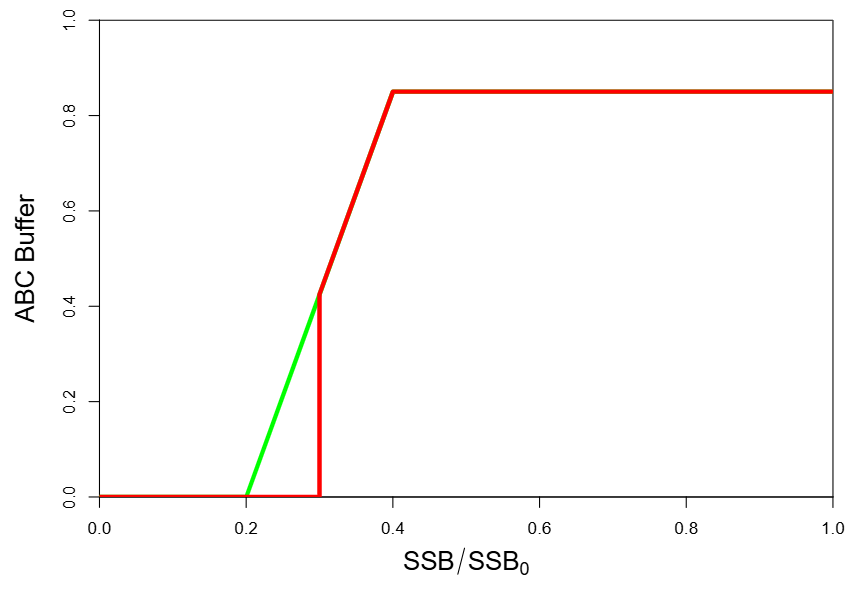
\includegraphics[width=0.7\textwidth]{images/ProtectionLevel.png}
    \caption{ABC buffer versus relative stock size. The green line shows the ABC buffer for a target reference point of 0.4 SSB\textsubscript{0}, a limit reference point of 0.2 SSB\textsubscript{0}, and default ABC buffer of 0.85. The red line matches the green line, except there is a protection level at 0.3 SSB\textsubscript{0}.}
    \label{fig:ProtectionLevel}
\end{figure}

\hypertarget{ForeSpawn}{}
\subsection[Forecast Recruitment Adjustment]{\protect\hyperlink{ForeSpawn}{Forecast Recruitment Adjustment}}
Recruitment during the forecast years sometimes needs to be set at a level other than that determined by the spawner-recruitment curve. One way to do this is by an environmental or block effect on the regime shift parameter. A more straightforward approach is now provided by the special forecast recruitment feature described here. There are 4 options provided for this feature. These are:

\begin{itemize}
	\item 0 = Do nothing: this is the default and will invoke no special treatment for the forecast recruitments.
	\item 1 = Multiplier on spawner-recruitment: the expected recruitment from the \gls{srr} is multiplied by this factor.
	\begin{itemize}
		\item This is a multiplier, so null effect comes from a value of 1.0.
		\item The order of operations is to apply the \gls{srr}, then the regime effect, then this special forecast effect, then bias adjustment, then the deviations.
		\item In the spawner recruit output of the \texttt{Report.sso} there are 4 recruitment values stored.
	\end{itemize}
	\item 2 = Multiplier on virgin recruitment: The virgin recruitment is multiplied by this factor.
	\begin{itemize}
		\item This is a multiplier, so null effect comes from a value of 1.0.
		\item The order of operations is to apply any environmental or block effects to $R_{0}$, then apply the special forecast effect, then bias adjustment, then the deviations.
		\item Note that environmental or block effects on $R_{0}$ are rare and are different from environment or block effects on the regime parameter.
	\end{itemize}
	\item 3 = Mean recent recruitment: calculate the mean recruitment and use it during the forecast period.
	\begin{itemize}
		\item Note that bias adjustment is not applied to this mean because the values going into the mean have already been bias adjusted.
	\end{itemize}
\end{itemize}

This feature affects the expected recruitment in all years after the last year of the main recruitment deviations. This means that if the last year of main recruitment deviations is before end year, then the last few recruitments, termed ``late'', are also affected by this forecast option. For example, option 3 would allow you to set the last 2 years of the time series and all forecast years to have recruitment equal to the mean recruitment for the last 10 years of the main recruitment era.

\pagebreak
